\documentclass{standalone}
\usepackage{tikz}
\usetikzlibrary{patterns, shapes.geometric}

\begin{document}

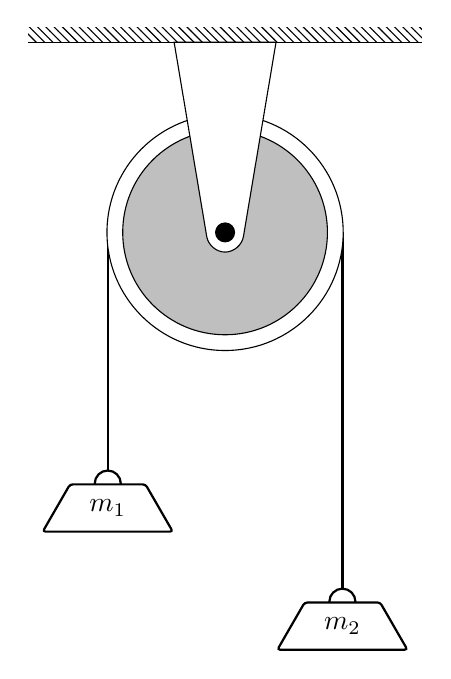
\begin{tikzpicture}

% Mass 1
\draw[thick] (1.49cm,0) -- ++(0,-5cm) node[draw=black,above=0.13cm,circle,fill=white](cM){}
node[draw=black,trapezium,rounded corners=1pt,fill=white,text=black, minimum height=0.6cm](M){$m_2$};

% Mass 2
\draw[thick] (-1.49cm,0) -- ++(0,-3.5cm) node[draw=black,above=0.13cm,circle,fill=white](cm){} node[draw=black,trapezium,rounded corners=1pt,fill=white,text=black, minimum height=0.6cm](m){$m_1$};

% Supporting structure
\fill[pattern= north west lines,] (-2.5,2.41) rectangle (2.5,2.6);
\draw(-2.5,2.41) -- (2.5,2.41);

% Pulley
\draw[fill=white] (0,0) circle (1.5cm); % Big circle
\draw[fill=lightgray] (0,0) circle (1.3cm); % Medium circle
\draw[fill=white] (75:2.5) to[rounded corners=0.2cm] (0.2,-0.25) to[rounded corners=0.2cm] (-0.2,-0.25) -- (105:2.5) -- cycle;
\draw[fill=black] (0,0) circle (0.12cm); % Axle circle

\end{tikzpicture}

\end{document}
